\documentclass[../main/thesis.tex]{subfiles}
\graphicspath{{/home/arefk/uio/MScThesis_AreKvanum2022_SeaIceML/thesis/physical_connections/figures/}}
\begin{document}

\section{Model explainability and physical connections}
\label{sec:physical-connections}
This section aims at presenting results intended to explain aspects of the deep learning system, such as predictor importance, how the model responds to the predictors as well as understanding how decisions where made by the deep learning system. This will be divided into three subsections. Firstly, model response to modified predictors will be measured. Secondly, individual predictions will be used to highlight how the model interprets the input data for decision-making. Thirdly, a case study will be conducted with the intent to relate the previous explainability results to a real world and in-distribution scenario.

\subsection{Predictor importance}
\label{sec:predictor-importance}
To measure the impact of each predictor, an experiment was conducted where the deep learning system was fitted to subset of the predictors, and the NIIEE with respect to the $(10\%)$ sea ice concentration contour was measured as a yearly mean value. The result of the experiment can be seen in Figure \ref{fig:leave-one-out}, where also persistence as well as an all predictor baseline was included for reference. From Figure \ref{fig:leave-one-out}, it can be seen that removing the recent sea ice chart as a predictor causes the deep learning system to achieve the highest NIIEE. Moreover, removing all AROME Arctic atmospheric predictors or the latest sea ice chart causes the deep learning system to perform worse than persistence for the 2022 test data period. Finally, removing 2-meter temperature seem to stochastically improve the forecast beyond the baseline with all predictors, as further indicated by training a new model without 2-meter temperature which achieves similar performance (orange line). 

\begin{figure}
    \centering
    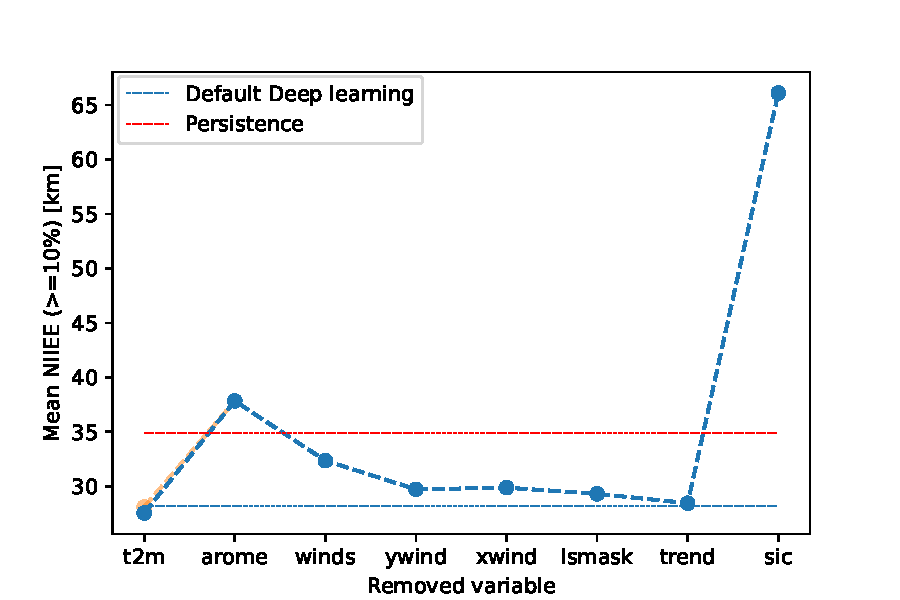
\includegraphics[width=\textwidth]{leave_one_out.pdf}
    \caption{\label{fig:leave-one-out}Yearly mean NIIEE for the $(\geq10\%)$ contour computed for deep learning systems where one (or a group) of the predictors have been removed. The red dashed line denotes the yearly mean NIIEE computed from persistence, whereas the blue dashed line denotes the yearly mean NIIEE for a benchmark deep learning model with all predictors. A two day lead time was considered. The orange mark and line seen for t2m is from an independent rerun. Trend refers to the OSI SAF linear sea ice trend. Winds refer to removing both the x and y component of the wind, whereas arome means removing all AROME Arctic atmospheric predictors.}
\end{figure}

Moreover, two more experiments where conducted to explore how sensitive a model fitted to all parameters are to perturbations in the input data. Firstly, it is noted that the model is trained on unaltered training and validation data, only the test dataset is permuted. The first experiment involves swapping all predictors with uniform noise between 0 and 1, which is the value range for the predictors after normalization (see section \ref{sec:dataloader}). The purpose of replacing a predictor with a uniform noise field is to study how much it alters the prediction of the model, i.e. if the model is strongly fitted to the predictor. The result of the first experiment is seen in figure \ref{fig:noisy}. Note that results regarding permuted SIC is not shown because the values [383, 439, 870, 851] are out of range. The SIC values are ordered in the same seasonal sequence as figure \ref{fig:noisy}.

Inspecting figure \ref{fig:noisy} (the caption) reveals that permuting SIC from the latest sea ice chart results in the highest NIIEE seasonal means. Following SIC, when swapping temperature out with random uniform noise, the NIIEE seasonal means are higher then persistence for both Summer and Autumn. 

\begin{figure}
    \centering
    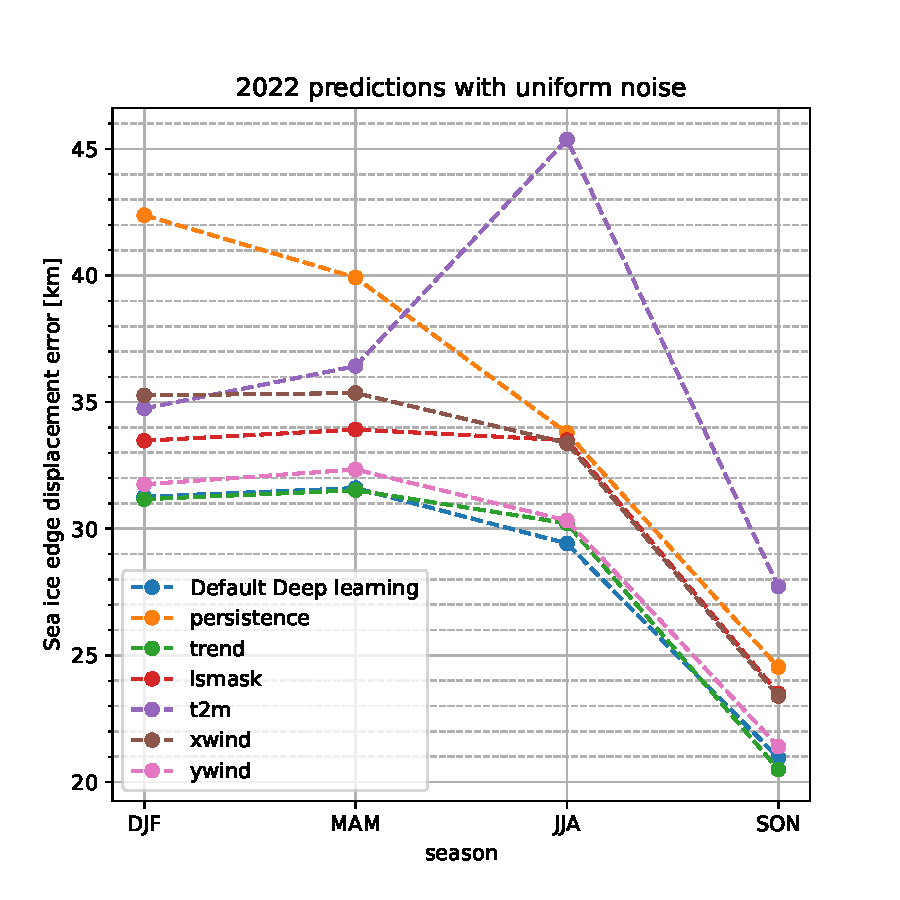
\includegraphics[width=\textwidth]{noisy.pdf}
    \caption{\label{fig:noisy}Seasonally distributed mean NIIEE for the $(\geq10\%)$ contour where each of the predictors have been swapped out with uniform noise between 0 and 1. Each colored line represent a variable that has been replaced, however the blue and orange line represent a no permuted baseline and persistence respectively. SIC is not shown because of out-of-range values, but results in the values [383, 439, 870, 851] distributed in the same seasonal sequence as the shown lines.}
\end{figure}

The second experiment conducted is similarly constructed to the previously described experiment of swapping out predictors with random noise, however instead of replacing each predictor with random noise each predictor have their 2022 test dataset sequence swapped. Thus, the distribution in which samples are drawn from is preserved. To account for seasonality, each prediction on the test data was repeated ten times for each predictor. The results of swapping predictor fields with fields from a different date is seen in figure \ref{fig:swapped}. As with figure \ref{fig:noisy}, SIC is not shown but results in the values [$186 \pm 13$, $225 \pm 29$, $266 \pm 36$, $230 \pm 29$] distributed in the same seasonal sequence as in figure \ref{fig:swapped}. The SIC values are not shown following the same reasoning for their exclusion in Figure \ref{fig:noisy}.

From figure \ref{fig:swapped}, it can be seen that swapping t2m is the only predictor which achieves a significantly higher NIIEE than persistence for the months JJA and SON. Moreover, for all seasons, all AROME Arctic predictors cause the model to have significantly higher NIIEE than the non-AROME Arctic predictors for all seasons. Figure \ref{fig:swapped} also shows that the swapped OSI SAF trend exerts no discernable standard deviation at all seasons.


\begin{figure}
    \centering
    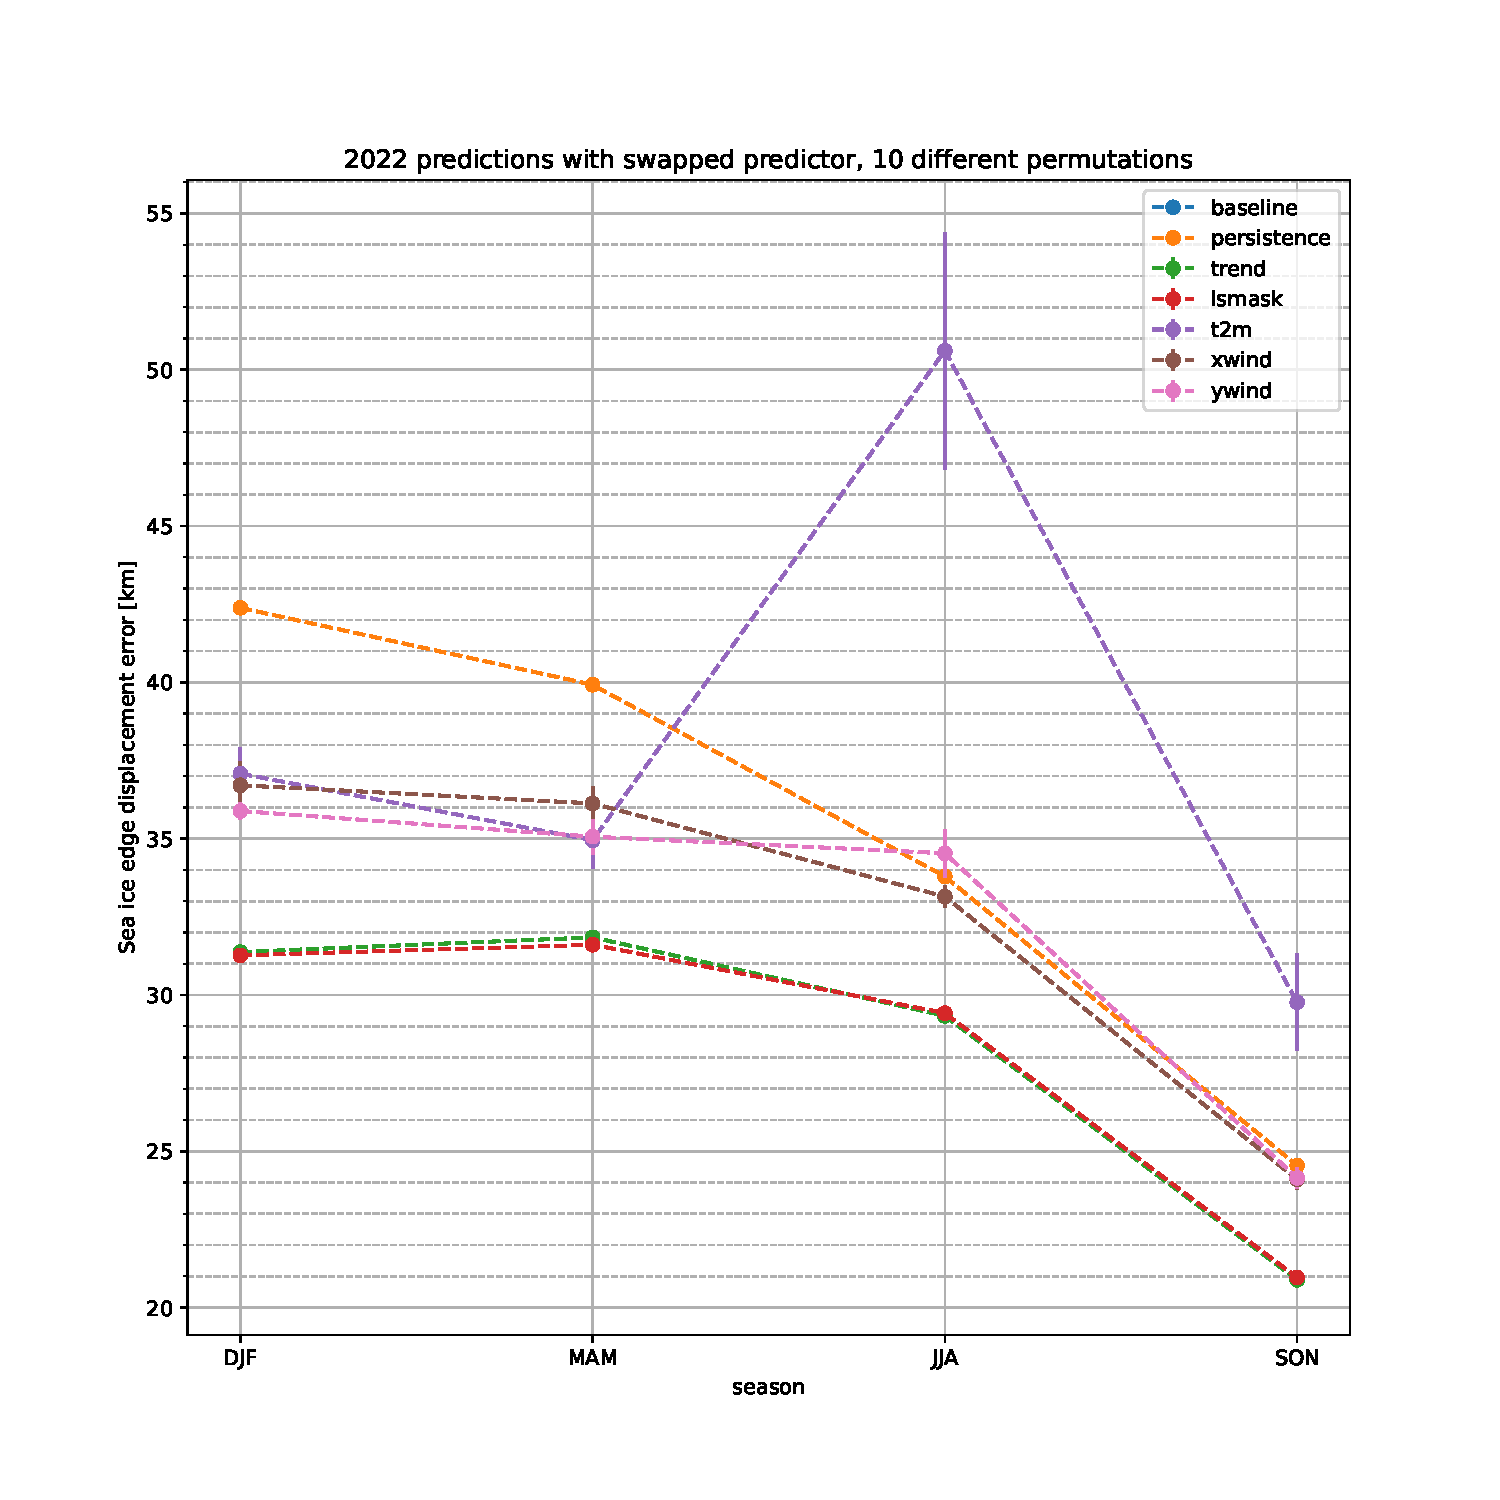
\includegraphics[width=\textwidth]{swapped.pdf}
    \caption{\label{fig:swapped}Seasonally distributed mean NIIEE for the $(\geq10\%)$ contour across 10 runs for each predictor, where each predictor have had their fields swapped internally. Each line represents one predictor. SIC is not shown because of out-of-range values, but it results in the values [$186 \pm 13$, $225 \pm 29$, $266 \pm 36$, $230 \pm 29$]. Results from the unperturbed Deep learning system are indistinguishable from the perturbed land-sea mask, since the land-sea mask is constant for all samples thus impossible to perturb.}
\end{figure}

\subsection{Synthetic AROME Artcic fields}
\label{sec:synthetic_preds}
Following the predictor importance experiments described previously in section \ref{sec:predictor-importance}, this section will describe an experiment which only targets the atmospheric predictors provided by AROME Arctic by constructing synthetic atmospheric fields and measuring how the deep learning system reacts. This experiment is similarly structured to a sensitivity experiment, which is a common technique to diagnose physical models in terms of how model parameters impact results e.g. \citep{Kim2006}. Firstly, a brief rundown of the synthetically created AROME Arctic fields and the experiment environment will be provided.

The deep learning model which is chosen, similar to previous results, is a the default Deep learning system trained on all predictors with a two day lead time. Four prediction dates covering months from different seasons have been chosen when measuring how the model responds to artificial AROME Arctic data, with the intent to also measure any seasonal variability in the responses. The chosen dates were 03rd March, 03rd June, 07th September and 07th December, with the dates referring to the valid date of the forecasts. Moreover, different synthetic fields were created.

When choosing values for the synthetic fields, it was decided to select values from the test dataset. This is done such that the values in the synthetic fields are consistent with the data used to test the Deep learning system, ensuring comparability of model response to the values. For 2-meter temperature, the minimum and maximum value in the test-dataset are (235K/$-38^{\circ}$C) and (299K/$26^{\circ}C$) respectively. Comparatively, for the x component of the winds the minimum value in the test-dataset is (-20m/s) and the maximum value is (24m/s). For the y component of the winds, the minimum and maximum values are (-26m/s) and (19m/s).

With regards to temperature, four fields were created where temperature increases linearly from one end of the domain to the other, starting at the lowest possible 2-meter temperature value in the test dataset and ending at the maximum 2-meter temperature value in the test dataset. Moreover, two homogenous fields containing only minimum or maximum values were created. For the winds, seven different fields were set up. The first field contains no wind in either x or y direction. Additionally, four fields where the wind was blowing in one direction (x or y, as well as positive or negative) were created. Finally, two fields where the winds were set to their maximum and minimum value in x and y at the same time was initiated.

Figure \ref{fig:synthetic_aa_niiee} shows how the model respond to synthetic AROME Arctic fields in terms of the NIIEE computed at the $(10\%)$ contour. From the figure, it can be seen that the model responds differently to the different fields for the inspected seasons. The synthetic fields tend to give the deep learning system higher NIIEE, except for two wind related fields for the september prediction. For all seasons, the highest NIIEE value is achieved with a synthetic temperature field, although having both the x and y winds at a maximum negative direction causes the highest NIIEE for all seasons compared to the other synthetic wind fields.

\begin{figure}
    \centering
    \begin{subfigure}[t]{.015\textwidth}
        a)
    \end{subfigure}
    \begin{subfigure}[t]{0.975\textwidth}
        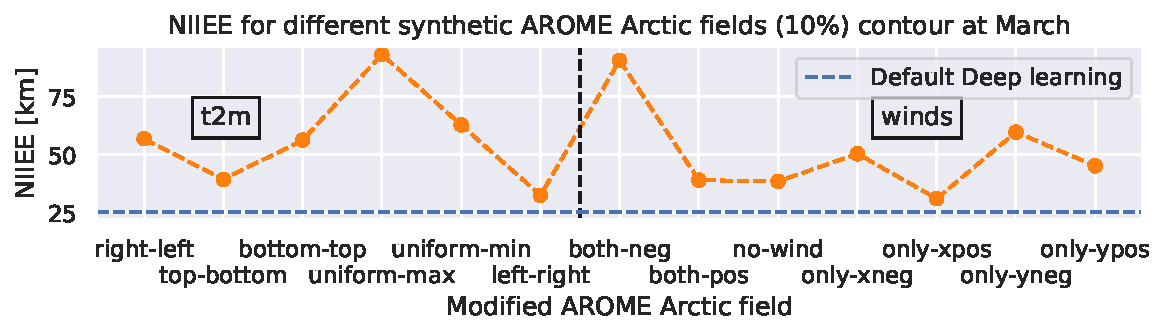
\includegraphics[width=\textwidth, valign = t]{NIIEE_03.pdf}
    \end{subfigure}
    \begin{subfigure}[t]{.015\textwidth}
        b)
    \end{subfigure}
    \begin{subfigure}[t]{0.975\textwidth}
        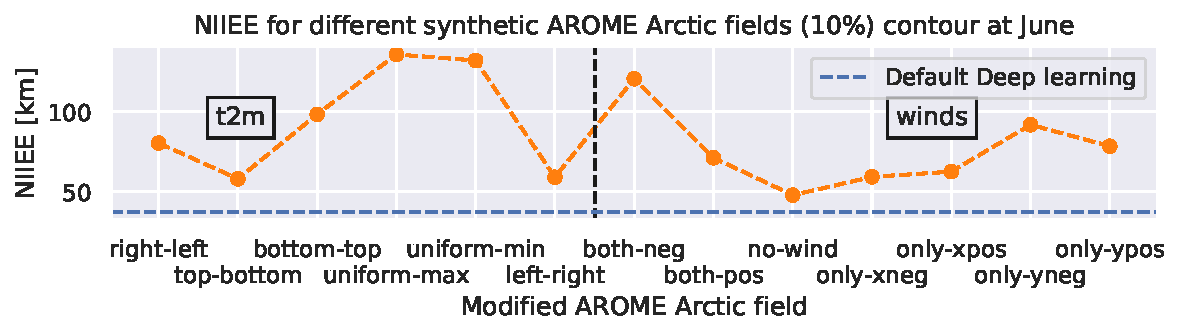
\includegraphics[width=\textwidth, valign = t]{NIIEE_06.pdf}
    \end{subfigure}
    \begin{subfigure}[t]{.015\textwidth}
        c)
    \end{subfigure}
    \begin{subfigure}[t]{0.975\textwidth}
        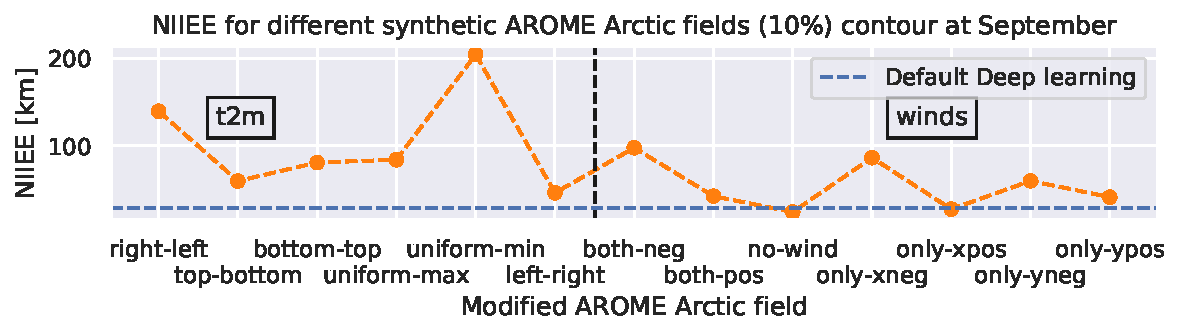
\includegraphics[width=\textwidth, valign = t]{NIIEE_09.pdf}
    \end{subfigure}
    \begin{subfigure}[t]{.015\textwidth}
        d)
    \end{subfigure}
    \begin{subfigure}[t]{0.975\textwidth}
        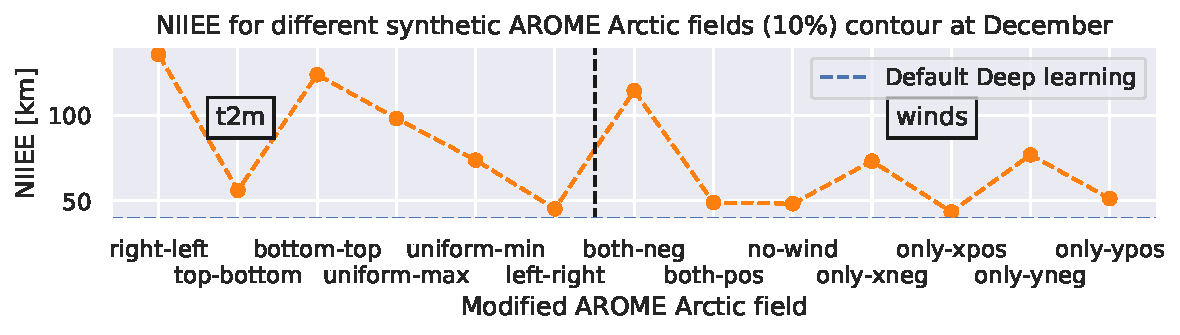
\includegraphics[width=\textwidth, valign = t]{NIIEE_12.pdf}
    \end{subfigure}
    \caption{\label{fig:synthetic_aa_niiee}NIIEE across different synthetic AROME Arctic fields measured at the 10\% contour for different seasons at 2-day lead time. The blue dashed line show the NIIEE value for the Default Deep learning system. The x axis summarizes the synthetic field. The vertical dashed line separates t2m and x,y-wind modifications.}
\end{figure}

Spatial errors are shown in figure \ref{fig:synthetic_aa_bias}, where some of the predictions made with the synthetic fields have been chosen. The top row of Figure \ref{fig:synthetic_aa_bias} shows two examples where synthetic wind fields have been constructed, and it is noted that a negative y-wind direction is towards the top of the domain. When both wind fields are pointed in a negative direction with maximum velocity from the test set, the sea ice concentration decreases towards lower categories as seen by the negative difference along the sea ice edge. With only x-wind in the positive direction with a maximum test set magnitude, a varied distribution of differences occurs along the sea ice edge, with an overall weak signature.

The lowermost row contains two prediction differences made with synthetic 2-meter temperature. The lower leftmost figure shows a consistent increase in sea ice concentration when the entire domain is covered by the lowest 2-meter temperature value found in the test dataset. Sea ice is forming in areas where it is usually not found during September, and sea ice is also forming along the coast of Norway. A similar response can be seen in the December prediction to the lower right, where temperature is linearly increasing from the minimum to maximum value of the test dataset from the bottom of the domain to the top of the domain. Sea ice is forming along the lower border of the domain, as well as above Russia. Moreover, following the temperature gradient, the sea ice tend to decrease as the 2-meter temperature increases. With the topmost past of the domain experiencing consistent melting.

\begin{figure}
    \centering
    \begin{subfigure}[t]{.03\textwidth}
        a)
    \end{subfigure}
    \begin{subfigure}[t]{.455\textwidth}
        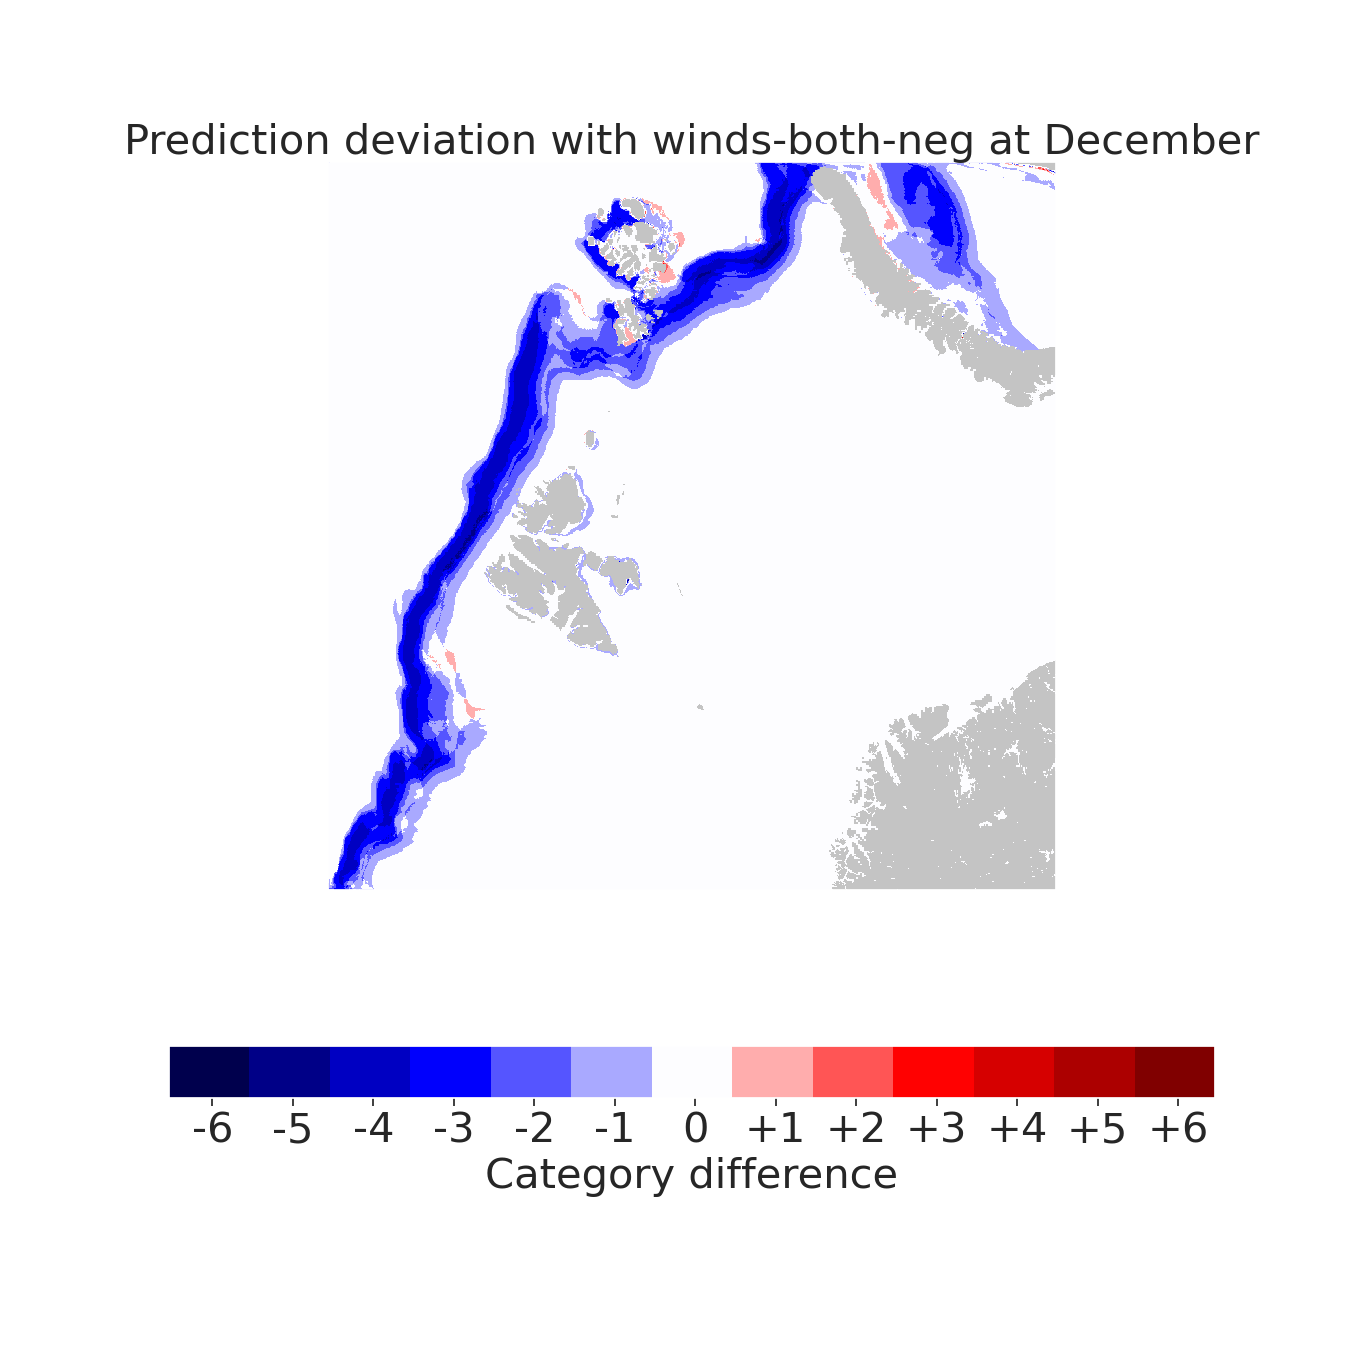
\includegraphics[width=\textwidth, valign=t]{bias_winds-both-neg}
    \end{subfigure}
    \begin{subfigure}[t]{.03\textwidth}
        b)
    \end{subfigure}
    \begin{subfigure}[t]{.455\textwidth}
        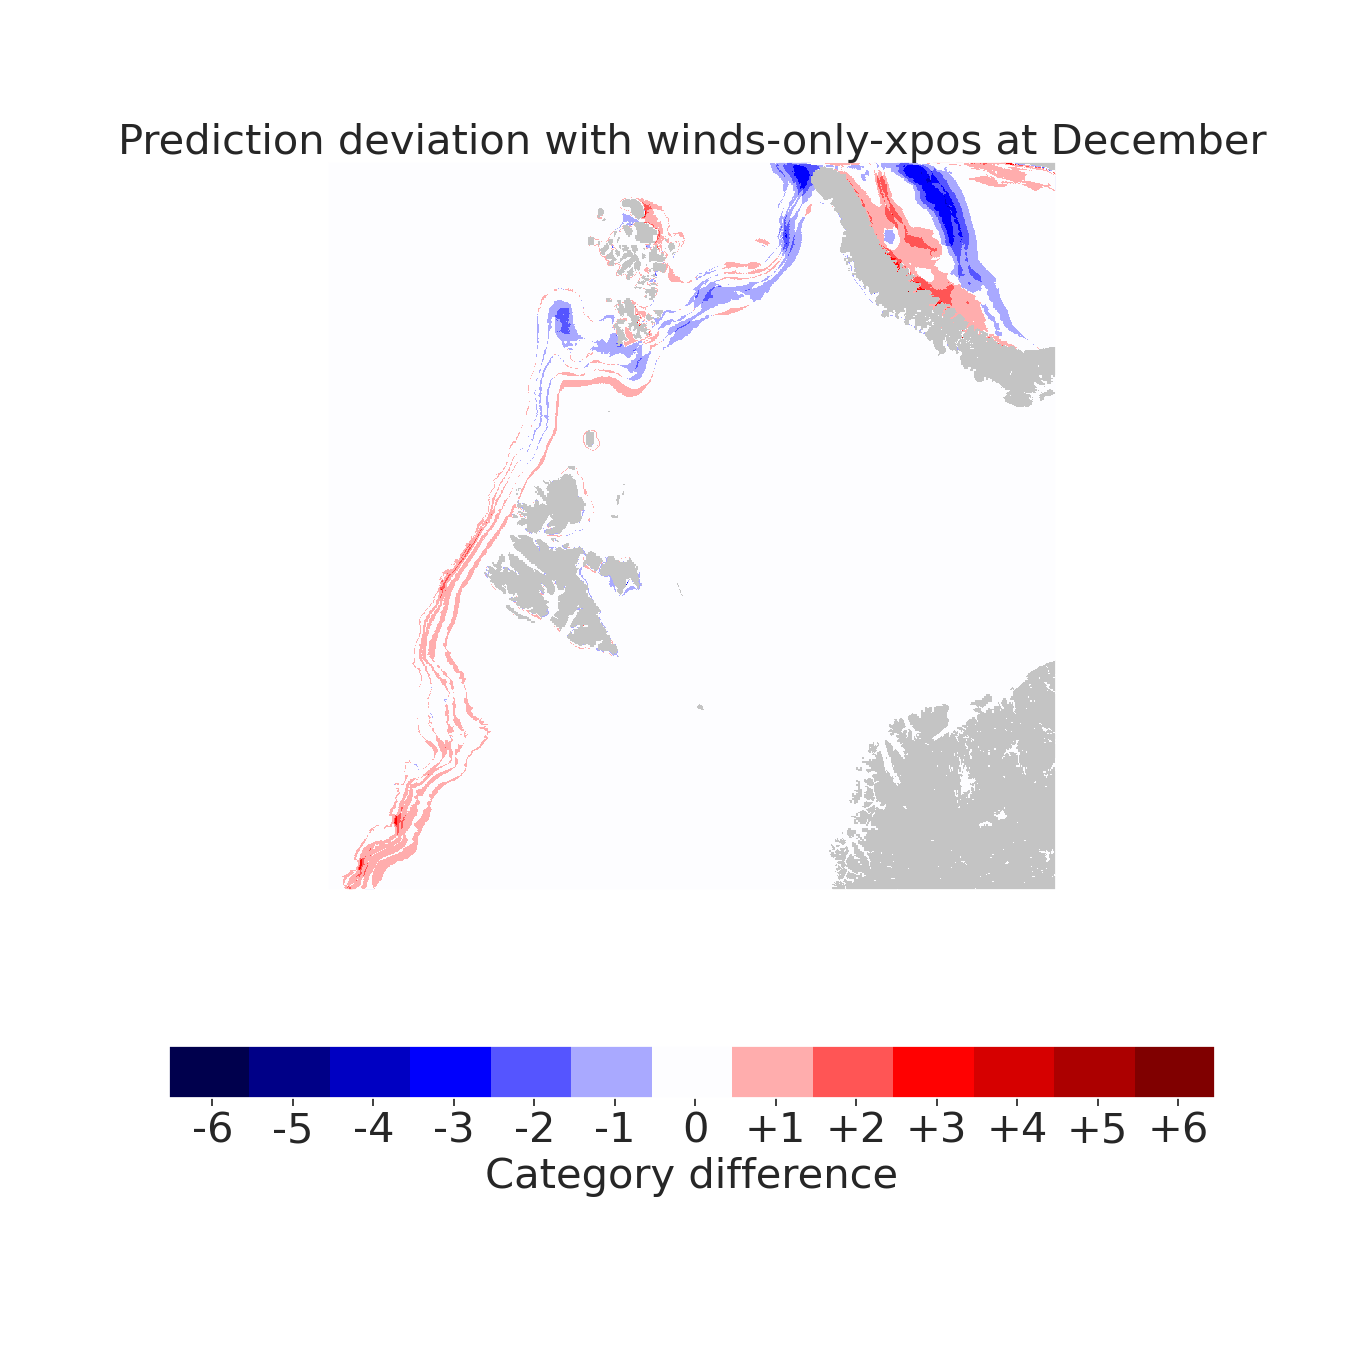
\includegraphics[width=\textwidth, valign=t]{bias_winds-only-xpos}
    \end{subfigure}
    \begin{subfigure}[t]{.03\textwidth}
        c)
    \end{subfigure}
    \begin{subfigure}[t]{.455\textwidth}
        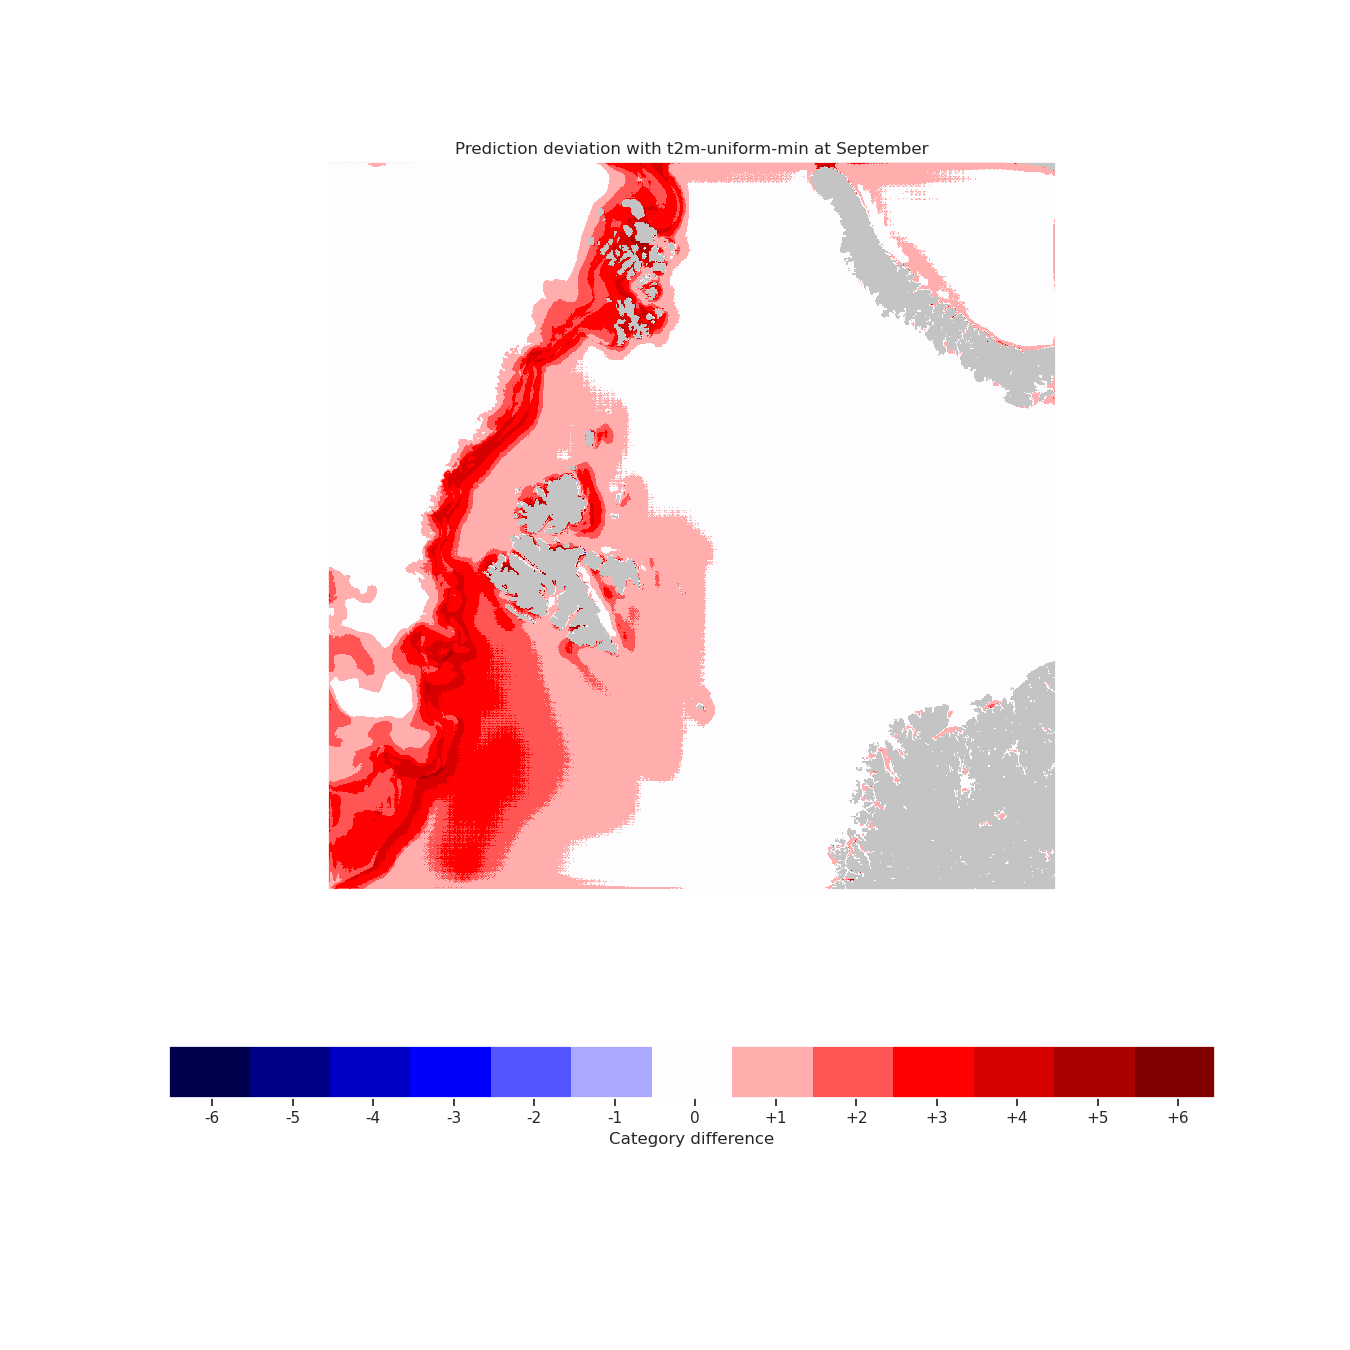
\includegraphics[width=\textwidth, valign=t]{bias_t2m-uniform-min}
    \end{subfigure}
    \begin{subfigure}[t]{.03\textwidth}
        d)
    \end{subfigure}
    \begin{subfigure}[t]{.455\textwidth}
        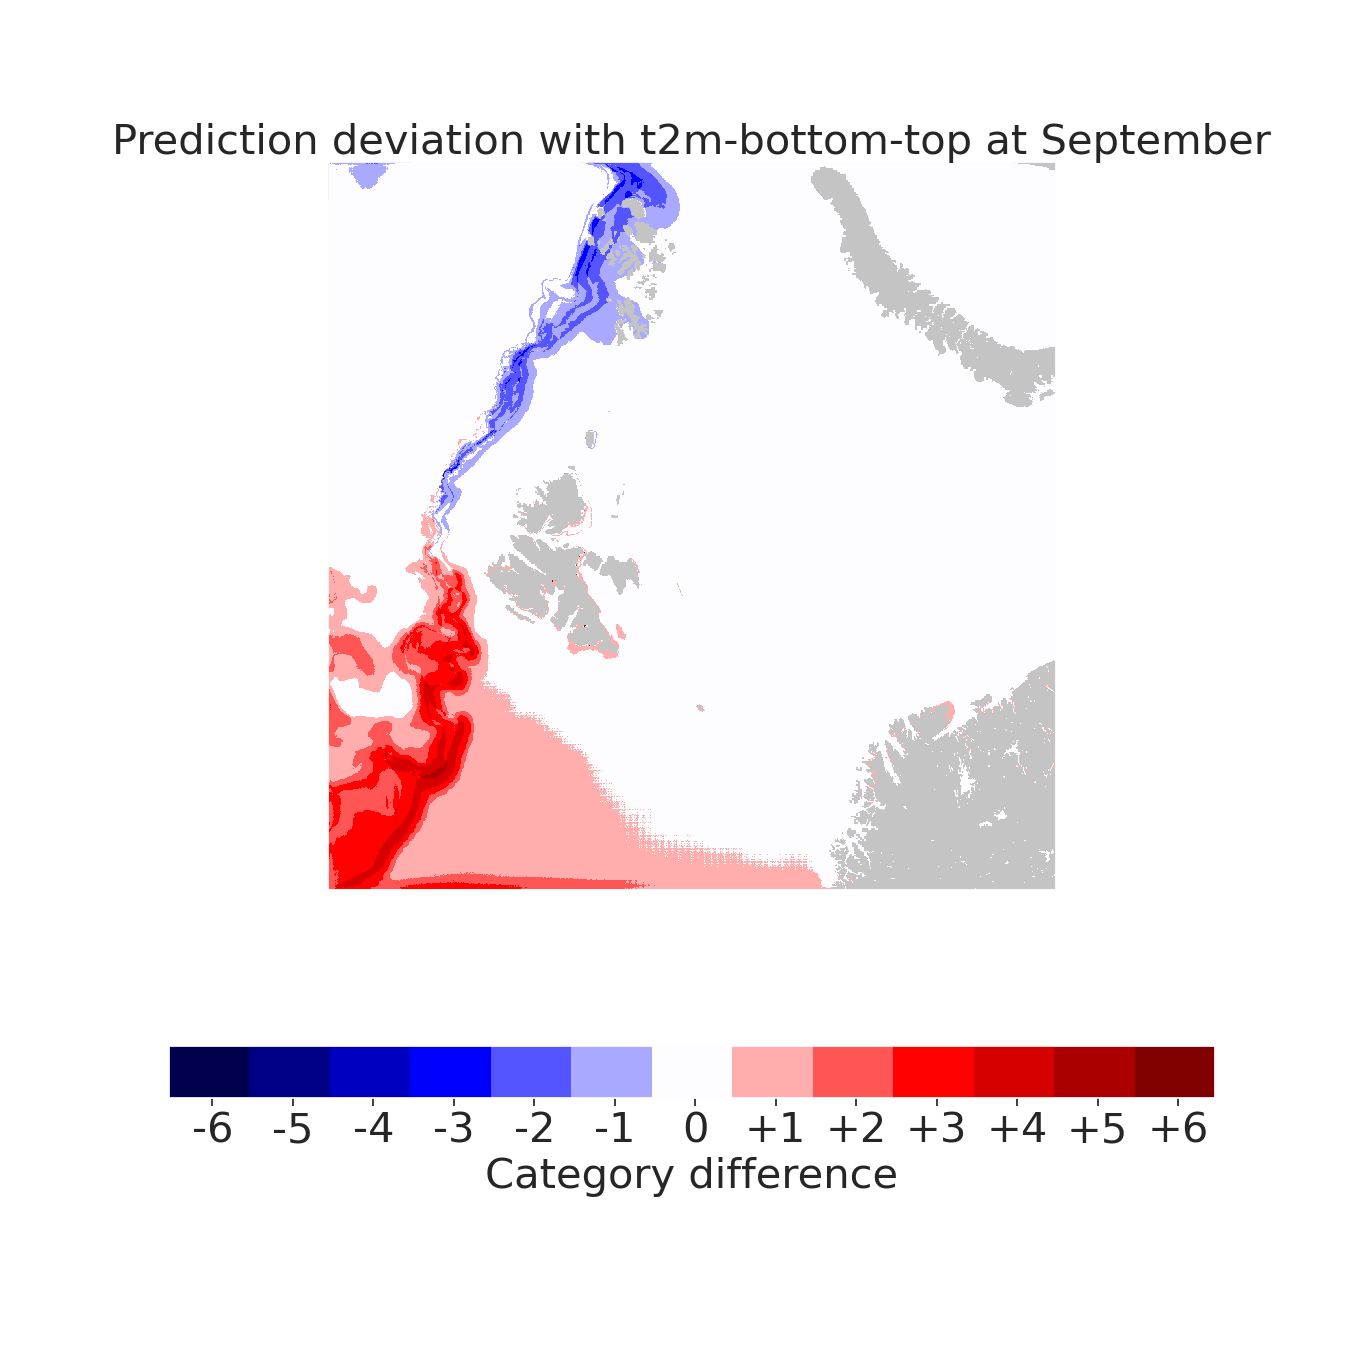
\includegraphics[width=\textwidth, valign=t]{bias_t2m-bottom-top}
    \end{subfigure}
    \caption{\label{fig:synthetic_aa_bias}Sea ice contour error with respective to the baseline prediction with no synthetic AROME Arctic field. The figure shows a selection of the synthetic fields, with the purpose of visualizing spatially how the deep learning system responds. In a) and b) prediction deviation from synthetic wind fields are shown. c) and d) show prediction deviation from synthetic 2-meter temperature fields.}
\end{figure}

The results that have been presented in Section \ref{sec:predictor-importance} and \ref{sec:synthetic_preds} all represent examples where the Deep learning system has been provided with out-of-distribution predictors. For Figure \ref{fig:noisy}, the sample is out-of-distribution since the modified predictor is composed by values drawn from a uniform distribution unlike the original unperturbed field. The samples used in Figure \ref{fig:swapped} are out-of-distribution since each sample contain a predictor which originates from another date. Finally, the synthetic AROME Arctic fields shown in Section \ref{sec:synthetic_preds} are also out-of-distribution due to the way they are constructed, since each synthetic predictor utilizes values ranging from the entirety if the test-dataset as well as spatially distributing values in an orderly fashion not seen in AROME Arctic. The above experiments are causing the Deep learning system to make predictions under very different conditions than what is present in the training dataset. This is generally not ideal, however the limits and precautions of the above experiments will be explored in the discussion.

\subsection{Understanding predictions}
Sections \ref{sec:predictor-importance} and \ref{sec:synthetic_preds} have presented results which attempt to explain the relationship between model performance and predictors. In the current section, predictions will be used to explain model decision-making through the use of segmentation gradient class activation maps (seg-GradCAM) \citep{Vinogradova2020} which was presented and described in section \ref{sec:seg-grad-cam}. Due to the formulation of the targets as cumulative contours (section \ref{sec:data_targets}), the gradient has to be computed from a single target output contour. Thus, each seg-GradCAM will only contain information related to wether a pixel was important for predicting the chosen cumulative contour, as a network used to create a segmentation gradient class activation map will be limited to predict only one cumulative contour. 

When creating seg-GradCAMs, only the final layer of the encoder will be considered following the recommendations made by \citet{Vinogradova2020}. This approach is also compliant with the originally proposed gradient class activation mapping (GradCAM) for classification tasks \citep{Selvaraju2016}, where it is recommended to compute the gradient with respect to the final convolutional layer. Since neither GradCAM or seg-GradCAM is intended for quantitative analysis, a case study approach is adopted where seg-GradCAMs from varying dates and contours will be inspected and compared. There are also no studies known to the author at the time of writing where results from gradCAM or seg-GradCAM have been applied to compute statistics.

Two experiments are conducted, one where the baseline model is compared against the model with reduced classes at different contours, and one where the baseline model is compared against the model trained without 2-meter temperature. For the first experiment where target contours are varied, 5th of January 2022 is chosen as the target date. For the second experiment where dates are varied. the same dates as those used in the synthetic AROME Arctic fields experiments are chosen, namely 3rd March, 3rd June, 7th September and 7th December. 

For all the following figures, a shared colorscale is used as values have been normalized between 0 and 1 following \citet{Vinogradova2020}. However, the actual values are not comparable, hence each seg-GradCAM shows the relative importance of each pixel for each contour. Furthermore, although \citet{Vinogradova2020} presents seg-GradCAM as a GradCAM computed from an arbitrary region of interest, for the following experiments the region of interest was defined as all pixels classified as part of the cumulative contour (both true and false positives). Furthermore, only non-zero values are shown.

A seg-GradCAM for varying target contours for the baseline model with a two day lead time is shown in figure \ref{fig:seg_base_cont}. The maps are spatially similar, although the intensity of the activated features tend to vary without a clear trend. The activated features seem to closely resemble the position of the sea ice edge. For figure \ref{fig:seg_base_cont} (a, b, c and d) the features with highest activation seem to be located in Frans Josef Land and Novaya Semlya (the latter not for (a)). 

\todo{Få inn hvilken date dette er}
\begin{figure}
    \centering
    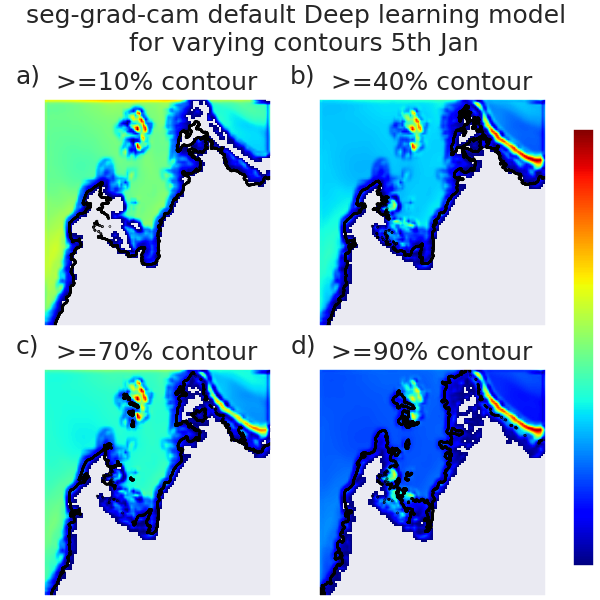
\includegraphics[width=0.49\textwidth]{baseline_contours}
    \caption{\label{fig:seg_base_cont}Segmentation class activation maps for varying target contours for the same date. The model used is the baseline model predicting with a two day lead time. The black line is the sea ice edge for the relevant contour from the input sea ice chart.}
\end{figure}

The seg-GradCAMs for the model without the $<10\%$ and $=100\%$ / fast-ice contour is shown in figure \ref{fig:seg_red_cont}. Each seg-GradCAM in figure \ref{fig:seg_red_cont} has significantly higher relative values compared to figure \ref{fig:seg_base_cont}. Moreover, whereas the highest activation values occurred over Frans Josef Land and Novaya Semlya for figure \ref{fig:seg_base_cont}, the opposite seems to be the effect for figure \ref{fig:seg_red_cont}. Furthermore, some spurious activations occur in figure \ref{fig:seg_red_cont} (a, b, c) located towards the lower right where mainland Norway is located.

\begin{figure}
    \centering
    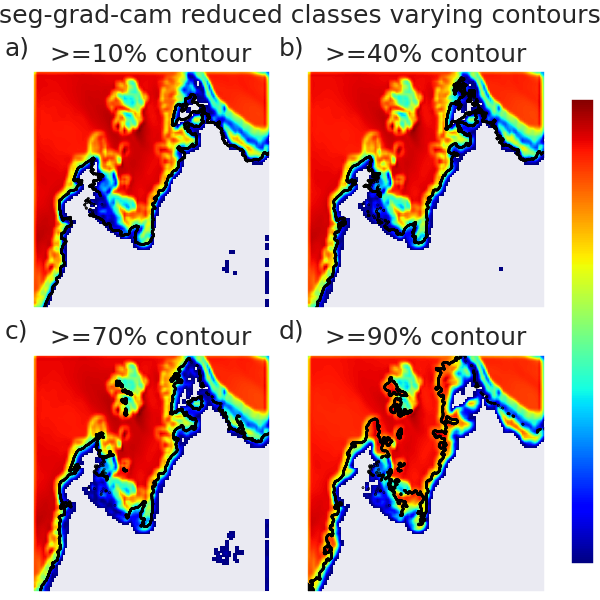
\includegraphics[width=0.49\textwidth]{reduced_classes_contours}
    \caption{\label{fig:seg_red_cont}Segmentation class activation maps for varying target contours for the same date. The model used is the reduced classes model predicting with a two day lead time. The black line is the sea ice edge for the relevant contour from the input sea ice chart.}
\end{figure}

The varying dates experiment for the baseline model is shown in figure \ref{fig:seg_base_dates}. As with figure \ref{fig:seg_base_cont}, the activated features tend to follow the sea ice edge, with no activated pixels located significantly outside of the sea ice edge. The relative value tend to be towards the upper limit, especially for figure \ref{fig:seg_base_dates} (b, c and d).

\begin{figure}
    \centering
    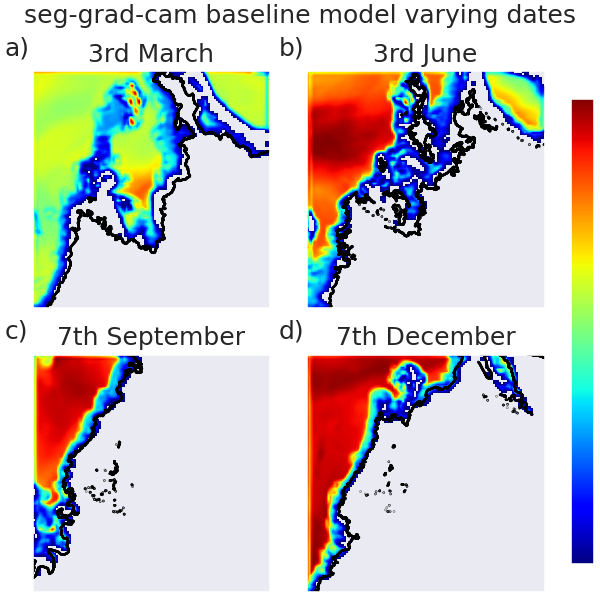
\includegraphics[width=0.49\textwidth]{baseline_dates}
    \caption{\label{fig:seg_base_dates}Segmentation class activation maps for varying dates for the same target contour. The model used is the baseline model predicting with a two day lead time. The black line is the sea ice edge for the relevant date from the input sea ice chart.}
\end{figure}

Finally, seg-GradCAM from the model trained without 2-meter temperature is shown in figure \ref{fig:seg_not2m_dates}. Compared to figure \ref{fig:seg_base_dates}, the relative values tend towards lower values. Contrary to Figure \ref{fig:seg_base_dates}, Figure \ref{fig:seg_not2m_dates} contains several large patches of activated features with low values located outside the border of the sea ice edge. For figure \ref{fig:seg_not2m_dates} (a and b), features located under Norway have been consistently activated. Moreover, for figure \ref{fig:seg_not2m_dates} (d) there appears to be activated features located in the inlet fjords of Svalbard, which is not seen in figure \ref{fig:seg_base_dates} (d).

\begin{figure}
    \centering
    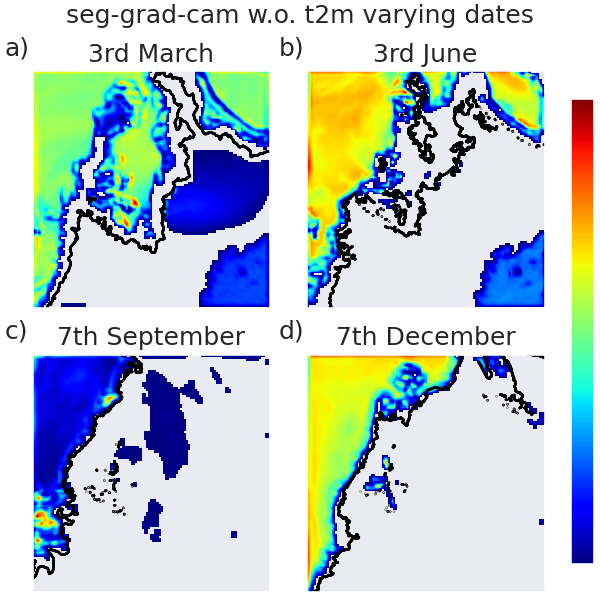
\includegraphics[width=0.49\textwidth]{not2m_dates}
    \caption{\label{fig:seg_not2m_dates}Segmentation class activation maps for varying dates for the same target contour. The model used is a model without 2-meter temperature as a predictor predicting with a two day lead time. The black line is the sea ice edge for the relevant date from the input sea ice chart.}
\end{figure}

\todo{Kanskje i appendix}
Figure \ref{fig:t2m_dates} show mean 2-meter temperature fields from AROME Arctic, used as predictors for the baseline model used in figure \ref{fig:seg_base_dates}. The sea ice chart is included to highlight the temperature-gradient in the scenes.

\begin{figure}
    \centering
    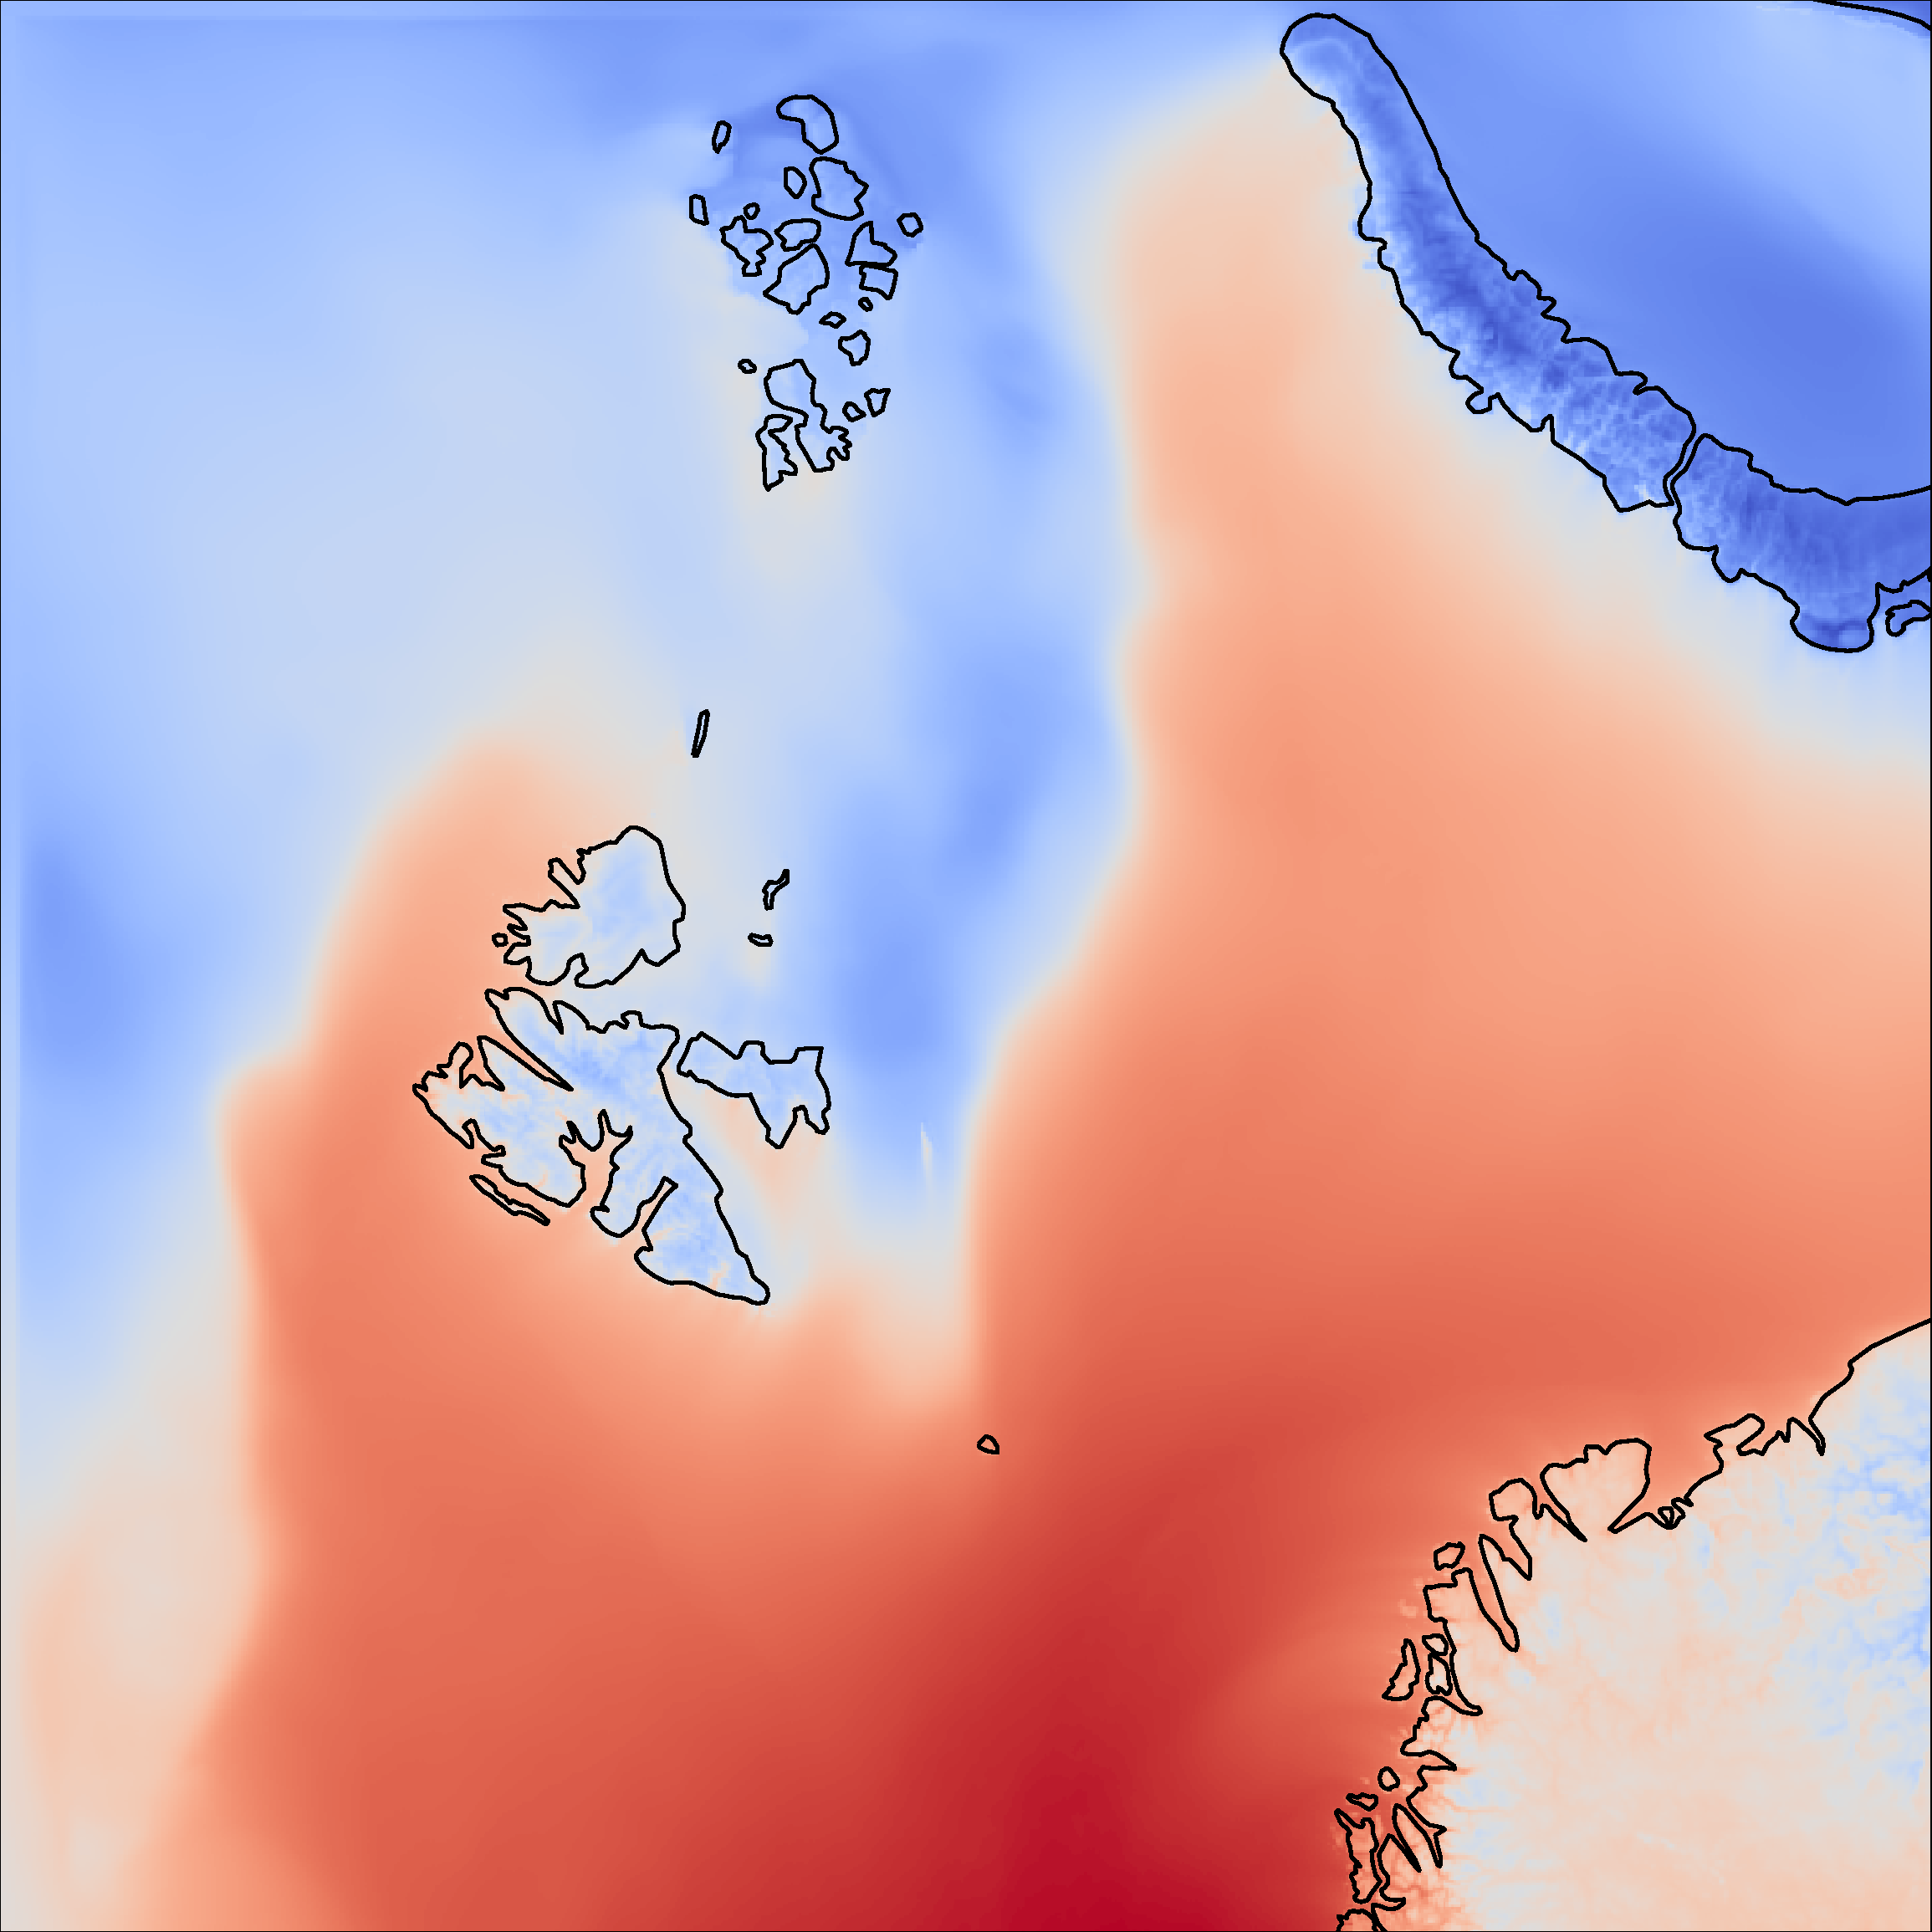
\includegraphics[width=0.49\textwidth]{t2m}
    \caption{\label{fig:t2m_dates}2-meter temperature mean fields used as predictor for the baseline model for varying dates. The black line is the sea ice edge for the relevant date from the input sea ice chart.}
\end{figure}

\subsection{Case study}
A case study is conducted for the date with the highest reported IIEE value from the baseline machine learning model, with a two day lead time. The motivation behind presenting a case study is to relate the previous model explainability results in sections \ref{sec:predictor-importance} and \ref{sec:synthetic_preds} to an example where the predictors are in-distribution, thus representing a possible model prediction. The day chosen was 18th of March 2022 (valid date), which implies that the deep learning forecast was initialized 16th of March 2022 (bulletin date). For the current date, the deep learning forecast achieved an NIIEE of 50.8km, with persistence achieving an NIIEE of 52.5km for the same date. The chosen date is 14th highest persistence NIIEE value. The purpose of including a case study is to understand if connections can be drawn between the input variables and output forecast, with the date of highest NIIEE for the test dataset chosen as it may be characterized by outlier like conditions compared to the mean annual NIIEE for the baseline model (28.2km). We believe that discussing an outlier prediction is instructive in terms of model explainability, as it may provide further insight into how the model responds to the input predictors. Furthermore, exploring the lower limits of model performance may reveal sea ice conditions in which the model is not well suited to predict.

The sea ice conditions for the bulletin and valid dates, as well as the sea ice forecast for the valid date is shown in figure \ref{fig:case_preds}. To aid in visualizing the differences between the sea ice concentration fields, the 10\% sea ice edge from the bulletin (figure \ref{fig:case_preds} (a)) is shown in figure \ref{fig:case_preds} (a, b and c). The sea ice edge for the valid sea ice field is only shown in figure \ref{fig:case_preds} (c) as the blue line. The two sea ice edges closely match along MIZ, however a major deviation between the two dates is the occurrence of a major loss of $10-30\%$ sea ice concentration north-east of Svalbard for the bulletin date sea ice chart (figure \ref{fig:case_preds} (b)). It is shown in figure \ref{fig:case_preds} (c) that the deep learning forecast has not predicted this particular loss of sea ice. For clarity, the sea ice chart in figure \ref{fig:case_preds} (a) was used as input for the deep learning system to make the forecast seen in figure \ref{fig:case_preds} (c).

\begin{figure}
    \centering
    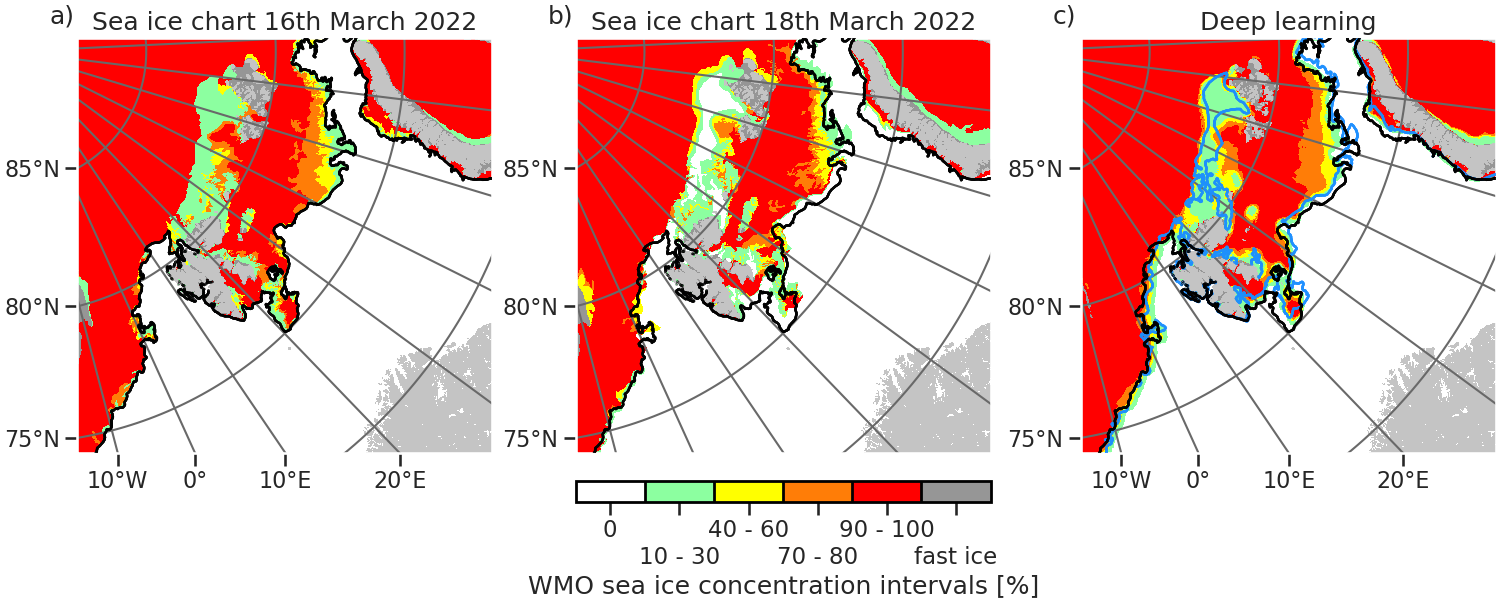
\includegraphics[width=\textwidth]{predictions}
    \caption{\label{fig:case_preds}Sea ice charts for the 16th (a) and 18th (b) of March 2022, with a deep learning prediction for 18th of March 2022 initialized 16th of March 2022 in (c). The black line is the sea ice edge for the sea ice chart in (a) and blue line is the sea ice edge for the sea ice chart in (b), both are thresholded by $10\%$ sea ice concentration. The $<10\%$ sea ice concentration contour is not shown.}
\end{figure}

The atmospheric predictors used to make the forecast in figure \ref{fig:case_preds} (c) are given in figure \ref{fig:case_atmos}. The fields shown are 2-meter temperature, as well as the x and y wind, which have been computed as two day mean fields between 16th of March 2022 18:00UTC and 18th of March 2022 12:00UTC following the approach for atmospheric predictor construction described in section \ref{sec:data_arome}. The 2-meter temperature field contains values $\sim 273$K, although significantly lower values are seen towards the top left of the scene (figure \ref{fig:case_atmos} (a)). The x-wind field mostly contains values centered about 0 m/s, although some outlier values are located along the north of Novaya Semlya blowing strongly towards its coast (figure \ref{fig:case_atmos} (b)). The y-wind component shows that the winds vary between being positively and negatively directed (in terms of the domain), although the y-wind along the sea ice edge (MIZ) tends to have a positive direction (figure \ref{fig:case_atmos} (c)).

\begin{figure}
    \centering
    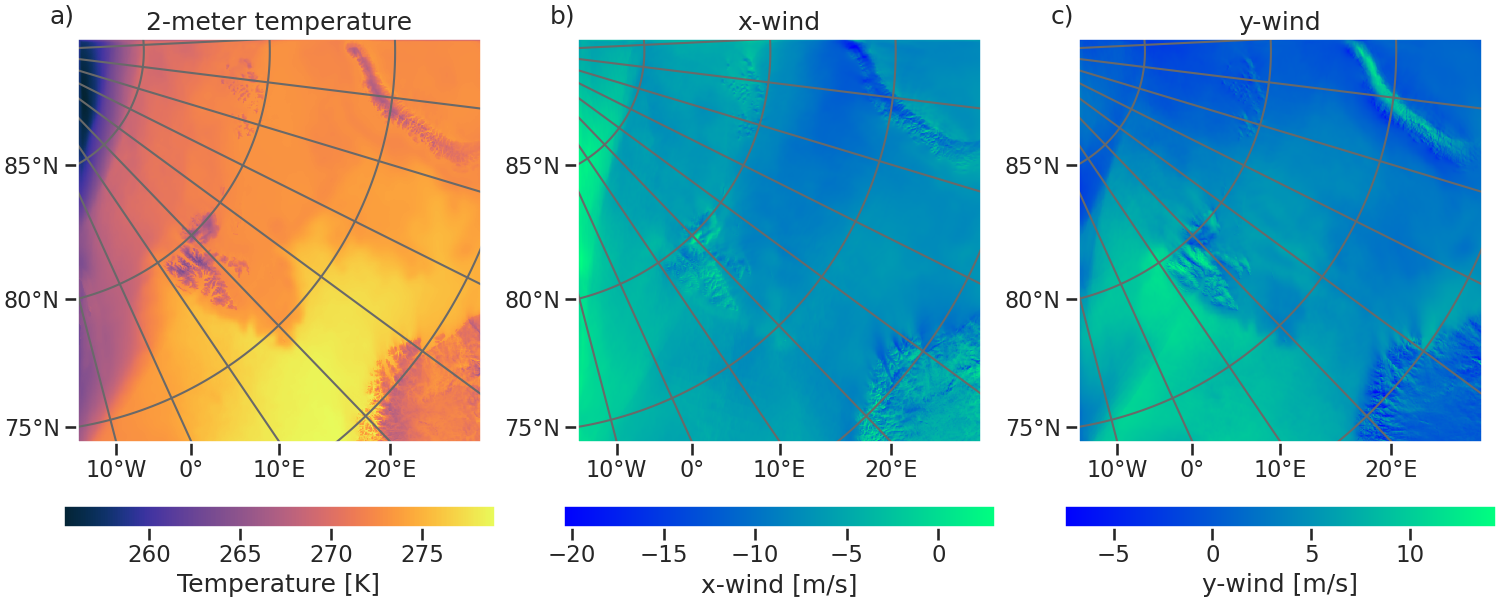
\includegraphics[width=\textwidth]{atmosphere}
    \caption{\label{fig:case_atmos}Atmospheric predictors for a sample initialized 16th of March 2022 for a two day lead time model. (a) is the two day mean AROME Arctic 2-meter temperature field. (b) and (c) are the two day mean x and y wind fields from AROME Arctic respectively.}
\end{figure}

The spatial distribution of deep learning forecast sea ice concentration overestimation and underestimation \citep{Goessling2016} with respect to the valid date sea ice chart is shown in figure \ref{fig:case_iiee}. Furthermore, areas where the two products agree are denoted as sea ice (positive agreement) and Ocean (negative agreement). The land sea mask is included in figure \ref{fig:case_iiee}, as the IIEE is computed without the land pixels. The deep learning forecast unresolved lack of sea ice north east of Svalbard (figure \ref{fig:case_preds} (c)) is clearly shown as overestimated sea ice concentration in figure \ref{fig:case_iiee}. Furthermore, figure \ref{fig:case_iiee} shows that the sea ice edge along the MIZ is overestimated towards the bottom of the domain, with some spurious underestimation located south of Svalbard. A consistent underestimation occurs towards the top of the domain, at the sea ice edge located opposite the northern edge of Novaya Semlya. Contrary, the sea ice concentration is overestimated along the coast of Novaya Semlya.

\begin{figure}
    \centering
    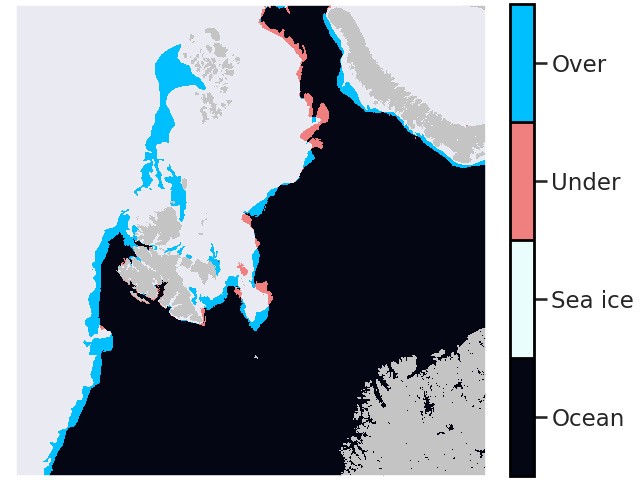
\includegraphics[width=\textwidth]{iiee}
    \caption{\label{fig:case_iiee}IIEE computed between the deep learning forecast valid 18th of March, initialized 16th of March 2022 and the sea ice chart for 18th of March 2022. Sea ice and Ocean denote true positives and true negative for the deep learning forecast.}
\end{figure}




\biblio
\end{document}